\documentclass{standalone}
\usepackage{tikz}
\usetikzlibrary{matrix, positioning, shapes, arrows, calc}

\usetikzlibrary{circuits.ee.IEC}

\tikzset{>=latex}

\begin{document}

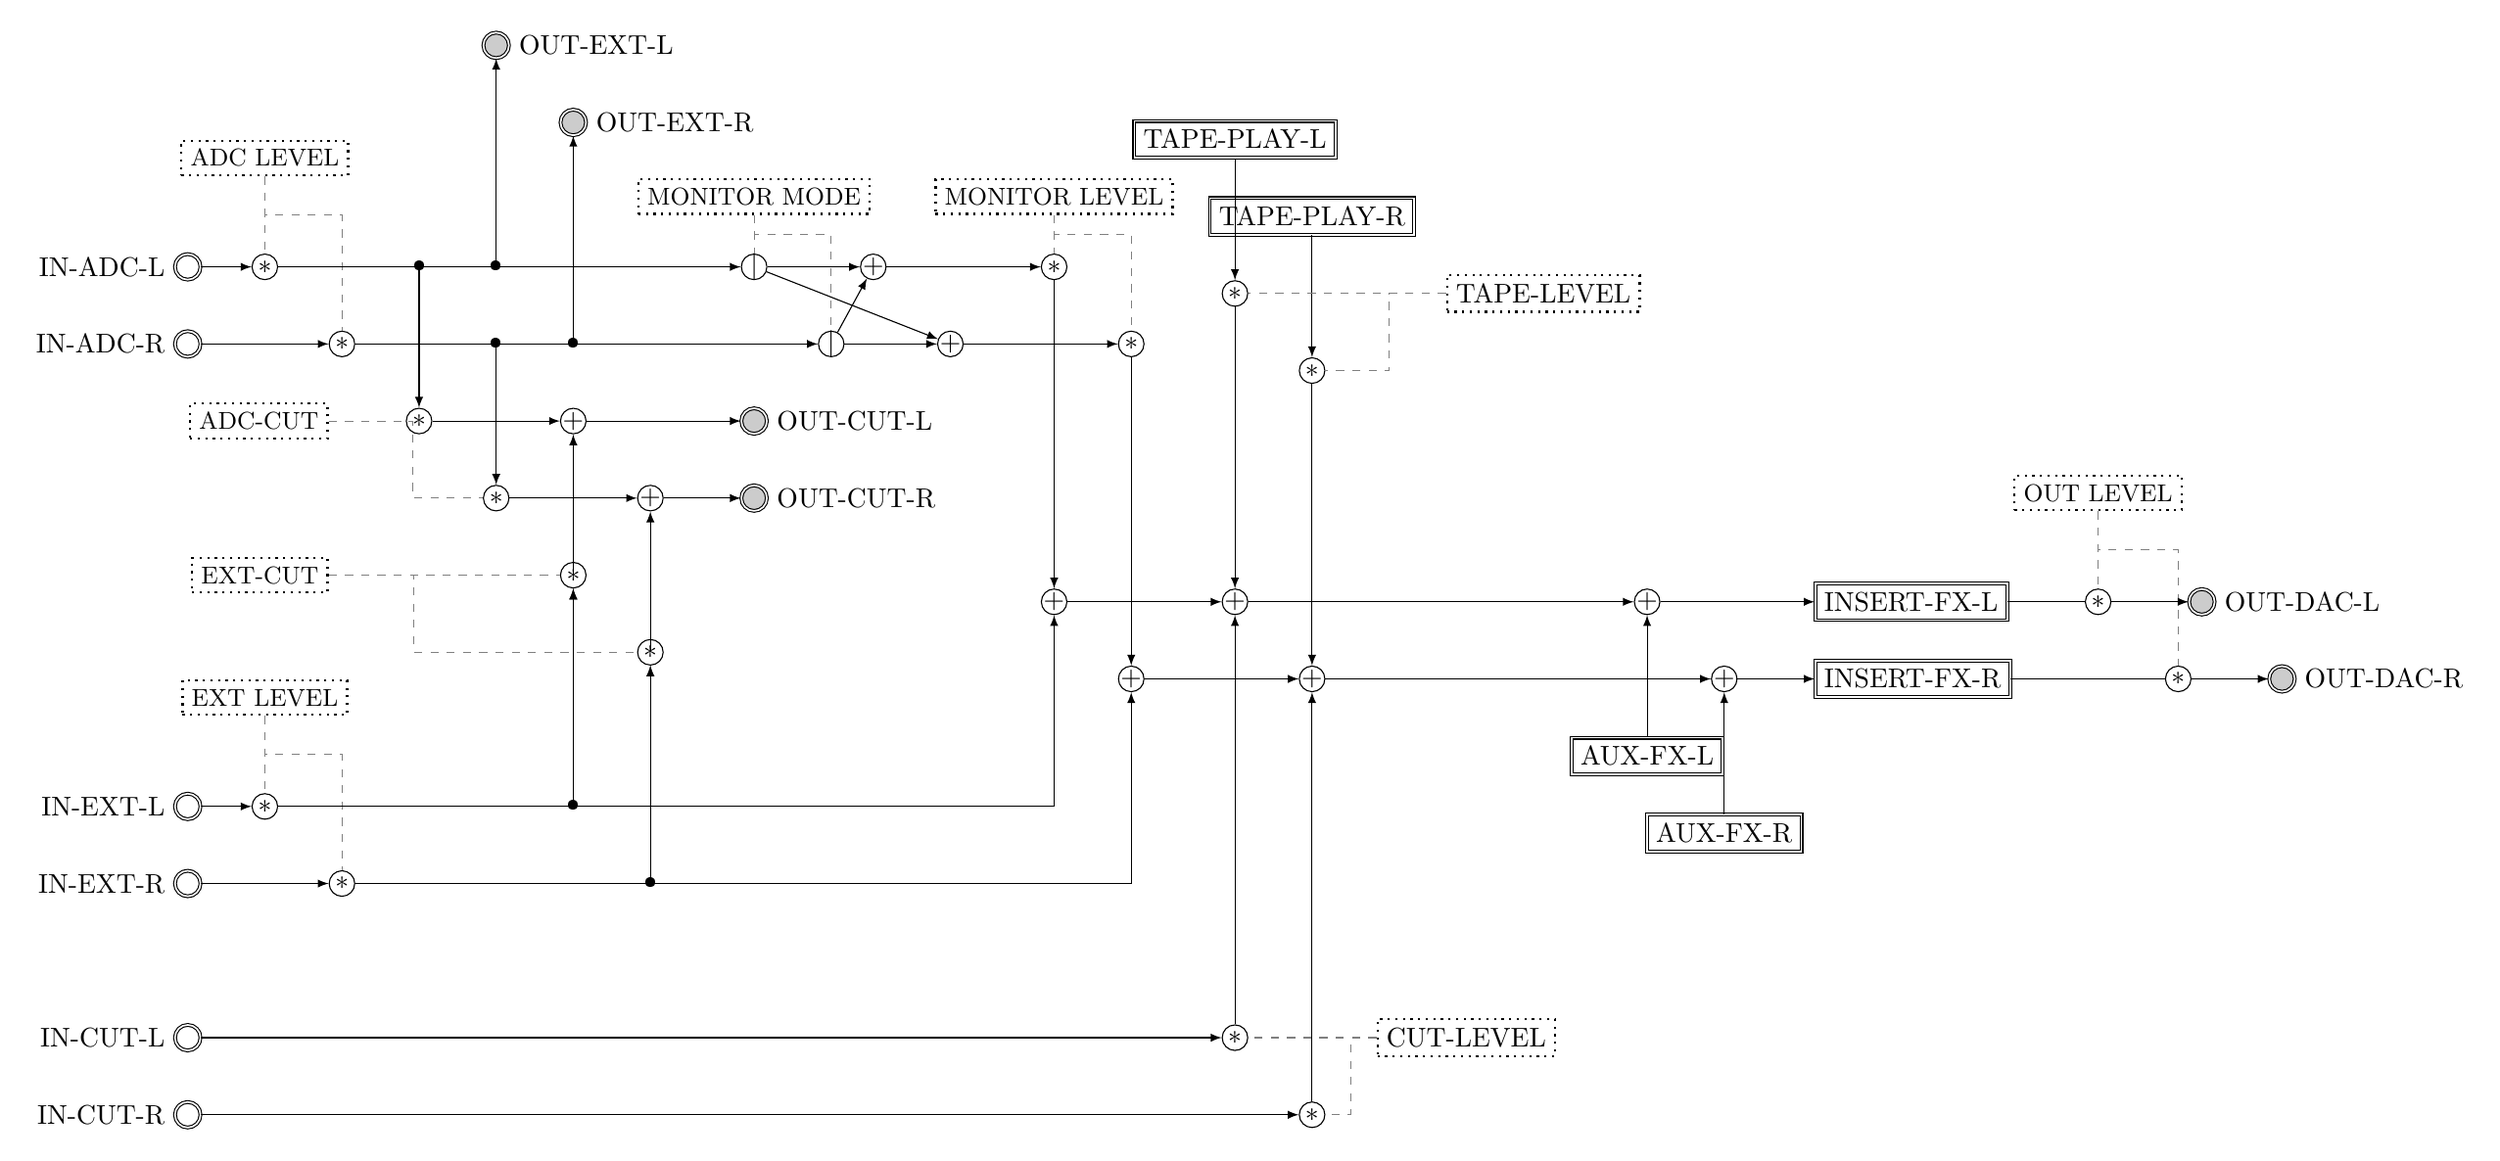
\begin{tikzpicture}

\tikzstyle{input}=[draw=black, circle, double, minimum size=1]
\tikzstyle{output}=[draw=black, circle, double, minimum size=1, fill=gray!40]
\tikzstyle{mul}=[draw=black, circle, minimum size=1, label=center:$\ast$]
\tikzstyle{add}=[draw=black, circle, minimum size=1, label=center:$+$]
\tikzstyle{or}=[draw=black, circle, minimum size=1, label=center:$|$]
\tikzstyle{bus}=[draw=black, rectangle]
\tikzstyle{param}=[draw=black, rectangle, dotted, thick]
\tikzstyle{bus}=[draw=black, rectangle, double]

%%%%%%%%%%%%%%%%%%%%%%%%%%%%
% input nodes
\node [input, label=left:IN-ADC-L] (in-adc-l) at (0, 12) {};
\node [input, label=left:IN-ADC-R] (in-adc-r) at (0, 11){};
\node [input, label=left:IN-EXT-L] (in-ext-l) at (0, 5) {};
\node [input, label=left:IN-EXT-R] (in-ext-r) at (0, 4) {};

\node [input, label=left:IN-CUT-L] (in-cut-l) at (0, 2) {};
\node [input, label=left:IN-CUT-R] (in-cut-r) at (0, 1) {};

%%%%%%%%%%%%%%%%%%
%% ADC section

% ADC levels
\node [mul] (adc-l-mul) at ($(in-adc-l)+(1,0)$) {};
\node [mul] (adc-r-mul) at ($(in-adc-r)+(2,0)$) {};
\draw [->] (in-adc-l) -- (adc-l-mul);
\draw [->] (in-adc-r) -- (adc-r-mul);
\node [param, above = 1 of adc-l-mul] (adc-level) {\small{ADC LEVEL}};
\draw [gray, dashed] (adc-level.south) -- ++(0, -0.5) -| (adc-l-mul);
\draw [gray, dashed] (adc-level.south) -| ++(0, -0.5) -| (adc-r-mul);

% ADC to EXT
\node (adc-l-ext-junc) at ($(adc-l-mul) + (3, 0)$) {\textbullet};
\node (adc-r-ext-junc) at ($(adc-r-mul) + (3, 0)$) {\textbullet};
\node [output, label=right:OUT-EXT-L, above=2.5 of adc-l-ext-junc] (out-ext-l) {}; 
\node [output, label=right:OUT-EXT-R, above=2.5 of adc-r-ext-junc] (out-ext-r) {}; 
\draw [->] (adc-l-ext-junc.center) -- (out-ext-l);
\draw [->] (adc-r-ext-junc.center) -- (out-ext-r);


% ADC to CUT
\node (adc-l-cut-junc) at ($(adc-l-mul) + (2, 0)$) {\textbullet};
\node (adc-r-cut-junc) at ($(adc-r-mul) + (2, 0)$) {\textbullet};
\node [mul] (adc-l-cut-mul) at ($(adc-l-cut-junc) - (0, 2)$) {};
\node [mul] (adc-r-cut-mul) at ($(adc-r-cut-junc) - (0, 2)$) {}; 
\node [param, left = 1 of adc-l-cut-mul] (adc-cut) {\small{ADC-CUT}};
\draw [->] (adc-l-cut-junc.center) -- (adc-l-cut-mul);
\draw [->] (adc-r-cut-junc.center) -- (adc-r-cut-mul);
\draw [gray, dashed] (adc-cut) -- ++(2, 0) -- (adc-l-cut-mul);
\draw [gray, dashed] (adc-cut) -- ++(2, 0) |- (adc-r-cut-mul);

%%%%%%%%%%%%%%%%%%%%%%%%%%
%% monitor section

% monitor mix
\node [or, right=6 of adc-l-mul, minimum size=0] (monitor-mix-in-l) {};
\node [or, right=6 of adc-r-mul, minimum size=0] (monitor-mix-in-r) {};
\node [add, right=1.2 of monitor-mix-in-l] (monitor-mix-out-l) {};
\node [add, right=1.2 of monitor-mix-in-r] (monitor-mix-out-r) {};	

\draw [->] (adc-l-mul) -- (monitor-mix-in-l);
\draw [->] (adc-r-mul) -- (monitor-mix-in-r);
\draw [->] (monitor-mix-in-l) -- (monitor-mix-out-l);
\draw [->] (monitor-mix-in-l) -- (monitor-mix-out-r);
\draw [->] (monitor-mix-in-r) -- (monitor-mix-out-l);
\draw [->] (monitor-mix-in-r) -- (monitor-mix-out-r);

\node [param, above = 0.5 of monitor-mix-in-l] (monitor-mode) {\small{MONITOR MODE}};
\draw [gray, dashed] (monitor-mode.south) -- ++(0,-0.25) -| (monitor-mix-in-l);
\draw [gray, dashed] (monitor-mode.south) -- ++(0,-0.25) -| (monitor-mix-in-r);

% monitor level
\node [mul, right=2 of monitor-mix-out-l] (monitor-mul-l) {};
\node [mul, right=2 of monitor-mix-out-r] (monitor-mul-r) {};
\draw [->] (monitor-mix-out-l) -- (monitor-mul-l);
\draw [->] (monitor-mix-out-r) -- (monitor-mul-r);
\node [param, above = 0.5 of monitor-mul-l] (monitor-level) {\small{MONITOR LEVEL}};
\draw [gray, dashed] (monitor-level.south) -- ++(0, -0.25) -| (monitor-mul-l);
\draw [gray, dashed] (monitor-level.south) -| ++(0, -0.25) -| (monitor-mul-r);

%%%%%%%%%%%%%%%%%%%%%%%%%%
%% insert FX, DAC
\node [add, below=4 of monitor-mul-l] (ins-in-l) {};
\node [add, below=4 of monitor-mul-r] (ins-in-r) {};
\node [add, right=2 of ins-in-l] (ins-in-2-l) {};
\node [add, right=2 of ins-in-r] (ins-in-2-r) {};
\node [add, right=5 of ins-in-2-l] (ins-in-3-l) {};
\node [add, right=5 of ins-in-2-r] (ins-in-3-r) {};

\node [bus, right =2 of ins-in-3-l] (ins-fx-l) {INSERT-FX-L};
\node [bus, right =1 of ins-in-3-r] (ins-fx-r) {INSERT-FX-R}; 
\node [mul, right =1 of ins-fx-l] (dac-mul-l) {};
\node [mul, right =2 of ins-fx-r] (dac-mul-r) {}; 
\node [output, right=1 of dac-mul-l, label=right:OUT-DAC-L] (out-dac-l){}; 
\node [output, right=1 of dac-mul-r, label=right:OUT-DAC-R] (out-dac-r){}; 

\node [param, above = 1 of dac-mul-l] (dac-level) {\small{OUT LEVEL}};
\draw [gray, dashed] (dac-level.south) -- ++(0, -0.5) -| (dac-mul-l);
\draw [gray, dashed] (dac-level.south) -| ++(0, -0.5) -| (dac-mul-r);

\draw [->] (ins-in-l) -- (ins-in-2-l);
\draw [->] (ins-in-r) -- (ins-in-2-r);
\draw [->] (ins-in-2-l) -- (ins-in-3-l);
\draw [->] (ins-in-2-r) -- (ins-in-3-r);
\draw [->] (ins-in-3-l) -- (ins-fx-l);
\draw [->] (ins-in-3-r) -- (ins-fx-r);
\draw [->] (ins-fx-l) -- (dac-mul-l) -- (out-dac-l);
\draw [->] (ins-fx-r) -- (dac-mul-r) -- (out-dac-r);
\draw [->] (monitor-mul-l) -- (ins-in-l);
\draw [->] (monitor-mul-r) -- (ins-in-r);

%%%%%%%%%%%%%%%%%%%%%%%%
%% EXT section

% EXT level
\node [mul] (ext-l-mul) at ($(in-ext-l)+(1,0)$) {};
\node [mul] (ext-r-mul) at ($(in-ext-r)+(2,0)$) {};
\draw [->] (in-ext-l) -- (ext-l-mul);
\draw [->] (in-ext-r) -- (ext-r-mul);
\node [param, above = 1 of ext-l-mul] (ext-level) {\small{EXT LEVEL}};
\draw [gray, dashed] (ext-level.south) -- ++(0, -0.5) -| (ext-l-mul);
\draw [gray, dashed] (ext-level.south) -| ++(0, -0.5) -| (ext-r-mul);

\draw [->] (ext-l-mul) -| (ins-in-l);
\draw [->] (ext-r-mul) -| (ins-in-r);

% EXT to CUT
\node (ext-l-cut-junc) at ($(ext-l-mul) + (4, 0)$) {\textbullet};
\node (ext-r-cut-junc) at ($(ext-r-mul) + (4, 0)$) {\textbullet};
\node [mul] (ext-l-cut-mul) at ($(ext-l-cut-junc) + (0, 3)$) {};
\node [mul] (ext-r-cut-mul) at ($(ext-r-cut-junc) + (0, 3)$) {}; 
\draw [->] (ext-l-cut-junc.center) -- (ext-l-cut-mul); 
\draw [->] (ext-r-cut-junc.center) -- (ext-r-cut-mul);
\node [param, left = 3 of ext-l-cut-mul] (ext-cut) {\small{EXT-CUT}};
\draw [->] (ext-l-cut-junc.center) -- (ext-l-cut-mul);
\draw [->] (ext-r-cut-junc.center) -- (ext-r-cut-mul);
\draw [gray, dashed] (ext-cut) -- ++(2, 0) -- (ext-l-cut-mul);
\draw [gray, dashed] (ext-cut) -- ++(2, 0) |- (ext-r-cut-mul);

%%%%%%%%%%%%
% CUT output
\node [add] (cut-sink-l) at ($(adc-l-cut-mul) + (2, 0)$) {};
\node [add] (cut-sink-r) at ($(adc-r-cut-mul) + (2, 0)$) {};
\draw [->] (adc-l-cut-mul) -- (cut-sink-l);
\draw [->] (adc-r-cut-mul) -- (cut-sink-r);
\draw [->] (ext-l-cut-mul) -| (cut-sink-l);
\draw [->] (ext-r-cut-mul) -| (cut-sink-r);

\node [output, label=right:OUT-CUT-L, right = 2 of cut-sink-l] (out-cut-l) {}; 
\node [output, label=right:OUT-CUT-R, right = 1 of cut-sink-r] (out-cut-r) {}; 
\draw [->] (cut-sink-l) -- (out-cut-l);
\draw [->] (cut-sink-r) -- (out-cut-r);

%%%%%%%%%%%%%
% CUT input

\node [mul] (cut-mul-l) at (ins-in-2-l |- in-cut-l) {};
\node [mul] (cut-mul-r) at (ins-in-2-r |- in-cut-r) {};
\draw [->] (cut-mul-l) -- (ins-in-2-l);
\draw [->] (cut-mul-r) -- (ins-in-2-r);

\node [param] (cut-level) at ($(cut-mul-l) + (3, 0)$) {CUT-LEVEL};
\draw [gray, dashed] (cut-level) -- ++(-1.5, 0) |- (cut-mul-l);
\draw [gray, dashed] (cut-level) -- ++(-1.5, 0) |- (cut-mul-r);

\draw [->] (in-cut-l) -- (cut-mul-l);
\draw [->] (in-cut-r) -- (cut-mul-r);

%%%%%%%%%%%%%%%%
%% TAPE section
\node [mul] (tape-mul-l) at ($(ins-in-2-l) + (0, 4)$) {};
\node [mul] (tape-mul-r) at ($(ins-in-2-r) + (0, 4)$) {};
\draw [->] (tape-mul-l) -- (ins-in-2-l);
\draw [->] (tape-mul-r) -- (ins-in-2-r);

\node [bus] (tape-play-l) at ($(tape-mul-l) + (0, 2)$) {TAPE-PLAY-L};
\node [bus] (tape-play-r) at ($(tape-mul-r) + (0, 2)$) {TAPE-PLAY-R};
\draw [->] (tape-play-l) -- (tape-mul-l);
\draw [->] (tape-play-r) -- (tape-mul-r);

\node [param] (tape-level) at ($(tape-mul-l) + (4, 0)$) {TAPE-LEVEL};
\draw [gray, dashed] (tape-level) -- ++(-2, 0) |- (tape-mul-l);
\draw [gray, dashed] (tape-level) -- ++(-2, 0) |- (tape-mul-r);


%%%%%%%%%%%%%%%%%
%% AUX section

\node [bus] (aux-fx-l) at ($(ins-in-3-l) + (0, -2)$) {AUX-FX-L};
\node [bus] (aux-fx-r) at ($(ins-in-3-r) + (0, -2)$) {AUX-FX-R};
\draw [->] (aux-fx-l) -- (ins-in-3-l);
\draw [->] (aux-fx-r) -- (ins-in-3-r);
\end{tikzpicture}

\end{document}
